\section{Problem 1}
\label{part1}
\subsection*{Question}
\begingroup
\begin{verbatim}
We know the result of the Karate Club (Zachary, 1977) split.
Prove or disprove that the result of split could have been predicted
by the weighted graph of social interactions.  How well does the
mathematical model represent reality?

Generously document your answer with all supporting equations, code,
graphs, arguments, etc.

Useful sources include:

* Original paper

http://aris.ss.uci.edu/~lin/76.pdf

* Slides

http://www-personal.umich.edu/~ladamic/courses/networks/si614w06/ppt/lecture18.ppt

http://clair.si.umich.edu/si767/papers/Week03/Community/CommunityDetection.pptx

* Code and data

http://networkx.github.io/documentation/latest/examples/graph/karate_club.html

http://nbviewer.ipython.org/url/courses.cit.cornell.edu/info6010/resources/11notes.ipynb

http://stackoverflow.com/questions/9471906/what-are-the-differences-between-community-detection-algorithms-in-igraph/9478989#9478989

http://stackoverflow.com/questions/5822265/are-there-implementations-of-algorithms-for-community-detection-in-graphs

http://konect.uni-koblenz.de/networks/ucidata-zachary

http://vlado.fmf.uni-lj.si/pub/networks/data/ucinet/ucidata.htm#zachary
\end{verbatim}
\endgroup

\newpage
\subsection*{Answer}
\begin{enumerate}
\item I had hard time understanding the concept of Karate Club. But after lot of research and reading the paper again and again I had a clear picture.
\item I figured that using R is a best when compared to python. There are different data sets available for Karate Club online. I downloaded ``karate.gml'' file and started working with that.
\item I loaded the ``karate.gml'' file into R and run through the program shown in Listing \ref{lst:q1codeR} at line 5. Lines 16-29 use the Girvan-Newman Betweenness Clustering Algorithm to slit the graph into various clusters. 
\item Using this implementation, I can split the group into as many clusters as I need by changing the threshold value. This algorithm goes through $16$ iterations before two groups are created. From this code Figures \ref{fig:before-split} and \ref{fig:after-split} were produced. 
\item Figure \ref{fig:before-split} shows the graph for the Karate Club's relationship prior to the split. According to Zachary's original paper, the node labeled $1$ represents ``Mr.Hi'' and the node labeled $34$ represent ``John A''. 
\item Figure \ref{fig:after-split} shows the graph of the Karate Club's relations after running the Girvan-Newman Betweenness Clustering Algorithm for Listing\ref{lst:q1codeR}
\item After the graph is produced I wanted to verify it so I did a little search online and realized that the weighted graph of karate Club data is available as predefined from the package ``igraphdata''. 
\item So I loaded this data into R and run through the program shown in Listing \ref{lst:q1codeR} instead of loading it form the ``karate.gml'' file. 
\item To my surprise the algorithm I used goes through $18$ iterations before two groups are created. From this data set Figure \ref{fig:karate-before-split} and \ref{fig:karate-after-split} were produced.
\item I checked with the code I wrote for the algorithm again and did a little more research and failed to find the reason behind different solutions. 
\item Figure\ref{fig:karate-before-split} shows the graph of the Karate Club's relation prior to the split and Figure\ref{fig:karate-after-split} shows the graph after the split.
\item Table \ref{tab:results} shows the results compared with Zachary's original predictions and the actual data. Column $5$ shows whether my Girvan-Newman Algorithm implementation resulted in a \emph{Hit} or \emph{Miss} for the data set loaded from the ``igraphdata'', where as column $7$ shows for the data set that is loaded from ``karate.gml'' file.
\item Zachary's Ford and Fulkerson procedure had a $\frac{33}{34} = 97\%$ success rate.  
\item My Girvan-Newman implementation has a $\frac{32}{34} = 94\%$ success rate for the data which loaded directly form the ``igraphdata'' package in R.
\item On the other had My Girvan-Newman implementation has a $\frac{31}{34} = 91\%$ success rate for the data which is loaded from the ``karate.gml'' file. 
\item So I preferred using the data that is loaded from the ``igraphdata'' for my future research.
\item My Girvan-Newman is $94\%$ success where as Zachary's Ford and Fulkerson is $97\%$, but my Girvan-Newman is still effective at predicting almost all of the group memberships. 
\item My implementation also predicted that individual $9$ would stay with Mr.Hi, which is missed by Zachary.
\item Either way, it can be proved that this split could have been predicted to greater the  $90\%$ accuracy using this data and these algorithms. 
\item In Zachary's paper he did not consider when the split could have been predicted. 
\item But by using the Girvan-Newman Algorithm we can find the earliest point at which a split can be predicted. And that can be done by looking into the number of iterations.
\item So by this we can say that the mathematical model (Girvan-Newman Algorithm) is $94\%$ success, so it's pretty much close to the reality. 

\end{enumerate}

\newpage

\begin{table}
\small
\begin{tabular}{ | c | p{2cm} | p{2cm} | p{2cm} | p{2cm} | p{2cm} | p{2cm} |}
\hline
Individual & Actual Group\newline Membership From Split & Zachary's Ford and Fulkerson Procedure Modeled Group\newline Membership From Split & Girvan-Newman Modeled Group\newline Membership From Split & Hit/Miss For Girvan-Newman& Girvan-Newman Modeled Group\newline Membership From Split
\newline (``karate.gml'')& Hit/Miss For Girvan-Newman\\
\hline
1 & Mr. Hi & Mr. Hi & Mr. Hi & Hit & Mr. Hi & Hit\\
\hline
2 & Mr. Hi & Mr. Hi & Mr. Hi & Hit & Mr. Hi & Hit\\
\hline
3 & Mr. Hi & Mr. Hi & Mr. Hi & Hit & John A & Miss\\
\hline
4 & Mr. Hi & Mr. Hi & Mr. Hi & Hit & Mr. Hi & Hit\\
\hline
5 & Mr. Hi & Mr. Hi & Mr. Hi & Hit & Mr. Hi & Hit\\
\hline
6 & Mr. Hi & Mr. Hi & Mr. Hi & Hit & Mr. Hi & Hit\\
\hline
7 & Mr. Hi & Mr. Hi & Mr. Hi & Hit & Mr. Hi & Hit\\
\hline
8 & Mr. Hi & Mr. Hi & Mr. Hi & Hit & Mr. Hi & Hit\\
\hline
9 & Mr. Hi & John A & Mr. Hi & Hit & John A & Miss\\
\hline
10 & John A & John A & Mr. Hi & Miss & John A & Hit\\
\hline
11 & Mr. Hi & Mr. Hi & Mr. Hi & Hit & Mr. Hi & Hit\\
\hline
12 & Mr. Hi & Mr. Hi & Mr. Hi & Hit & Mr. Hi & Hit\\
\hline
13 & Mr. Hi & Mr. Hi & Mr. Hi & Hit & Mr. Hi & Hit\\
\hline
14 & Mr. Hi & Mr. Hi & Mr. Hi & Hit & John A & Miss\\
\hline
15 & John A & John A & John A & Hit & John A & Hit\\
\hline
16 & John A & John A & John A & Hit & John A & Hit\\
\hline
17 & Mr. Hi & Mr. Hi & Mr. Hi & Hit & Mr. Hi & Hit\\
\hline
18 & Mr. Hi & Mr. Hi & Mr. Hi & Hit & Mr. Hi & Hit\\
\hline
19 & John A & John A & John A & Hit & John A & Hit\\
\hline
20 & Mr. Hi & Mr. Hi & Mr. Hi & Hit & Mr. Hi & Hit\\
\hline
21 & John A & John A & John A & Hit & John A & Hit\\
\hline
22 & Mr. Hi & Mr. Hi & Mr. Hi & Hit & Mr. Hi & Hit\\
\hline
23 & John A & John A & John A & Hit & John A & Hit\\
\hline
24 & John A & John A & John A & Hit & John A & Hit\\
\hline
25 & John A & John A & John A & Hit & John A & Hit\\
\hline
26 & John A & John A & John A & Hit & John A & Hit\\
\hline
27 & John A & John A & John A & Hit & John A & Hit\\
\hline
28 & John A & John A & John A & Hit & John A & Hit\\
\hline
29 & John A & John A & John A & Hit & John A & Hit\\
\hline
30 & John A & John A & John A & Hit & John A & Hit\\
\hline
31 & John A & John A & John A & Hit & John A & Hit\\
\hline
32 & John A & John A & Mr. Hi & Miss & John A & Hit\\
\hline
33 & John A & John A & John A & Hit & John A & Hit\\
\hline
34 & John A & John A & John A & Hit & John A & Hit\\
\hline
\end{tabular}
\caption{Results of Split, as predicted by my Girvan-Newman Implementation and also compared to Zachary's predictions and the actual data}
\label{tab:results}
\end{table}



\newpage
\lstinputlisting[language=R,frame=single,caption={R program for Girvan \& Newman Betweenness Clustering shown in Figures \ref{fig:before-split} and \ref{fig:after-split}},label=lst:q1codeR,captionpos=b,numbers=left,showspaces=false,showstringspaces=false,basicstyle=\footnotesize]{R/karate.R}

\begin{figure}[h]
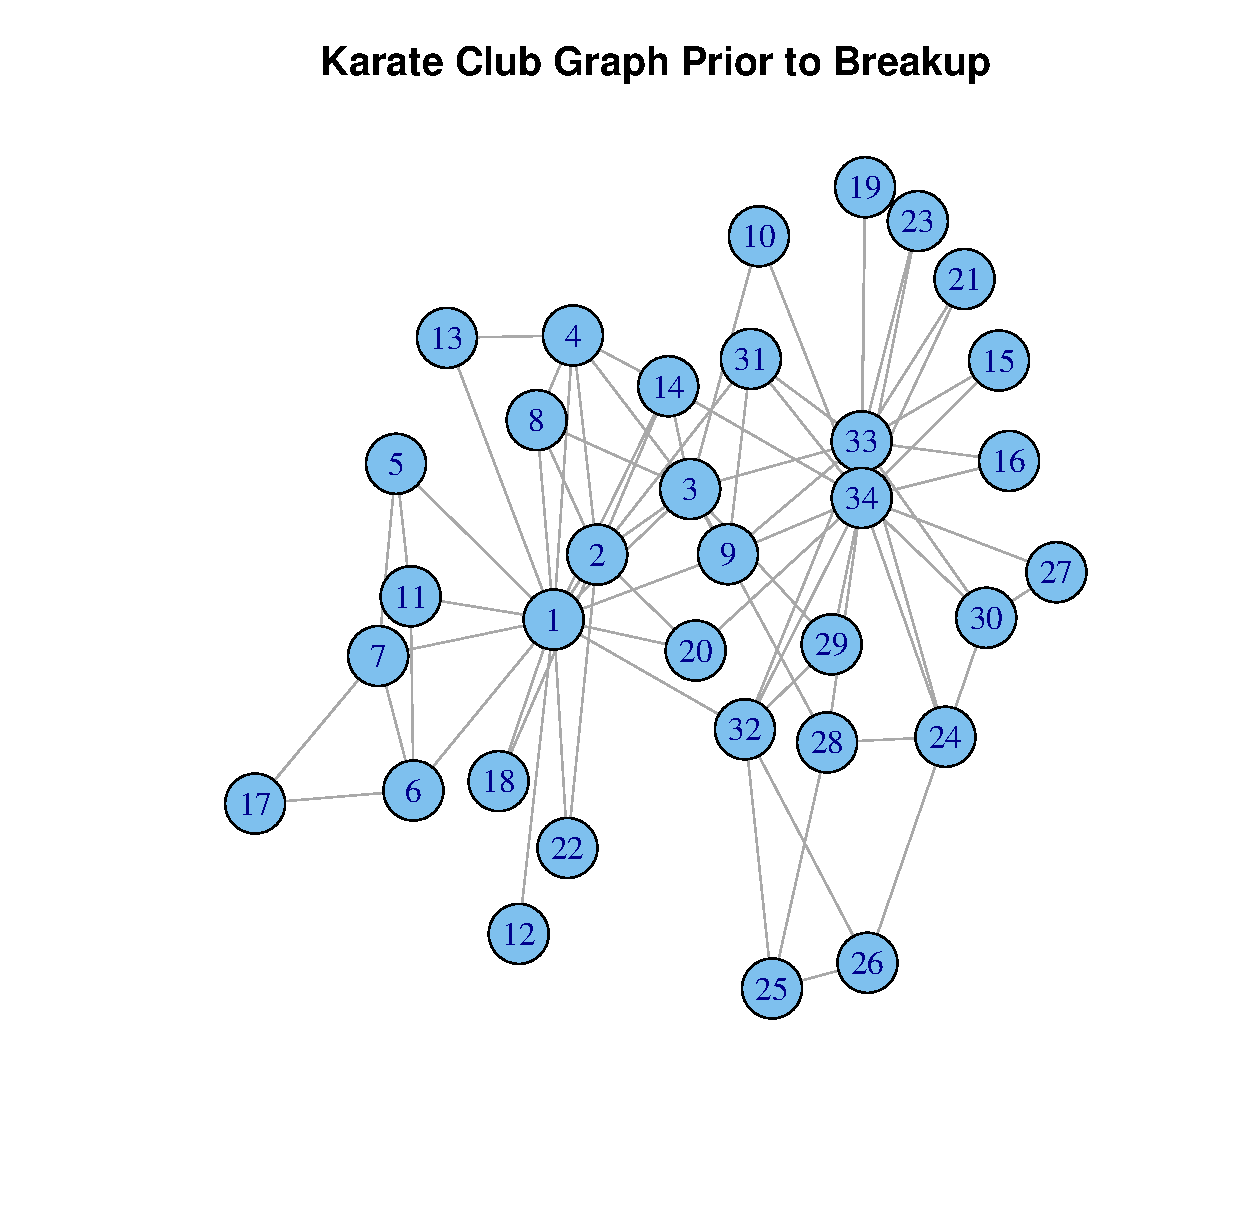
\includegraphics[scale=0.6]{R/kclub-gml.pdf}
\caption{Karate Club Graph prior to split for ``karate.gml''}
\label{fig:before-split}
\end{figure}

\begin{figure}[h]
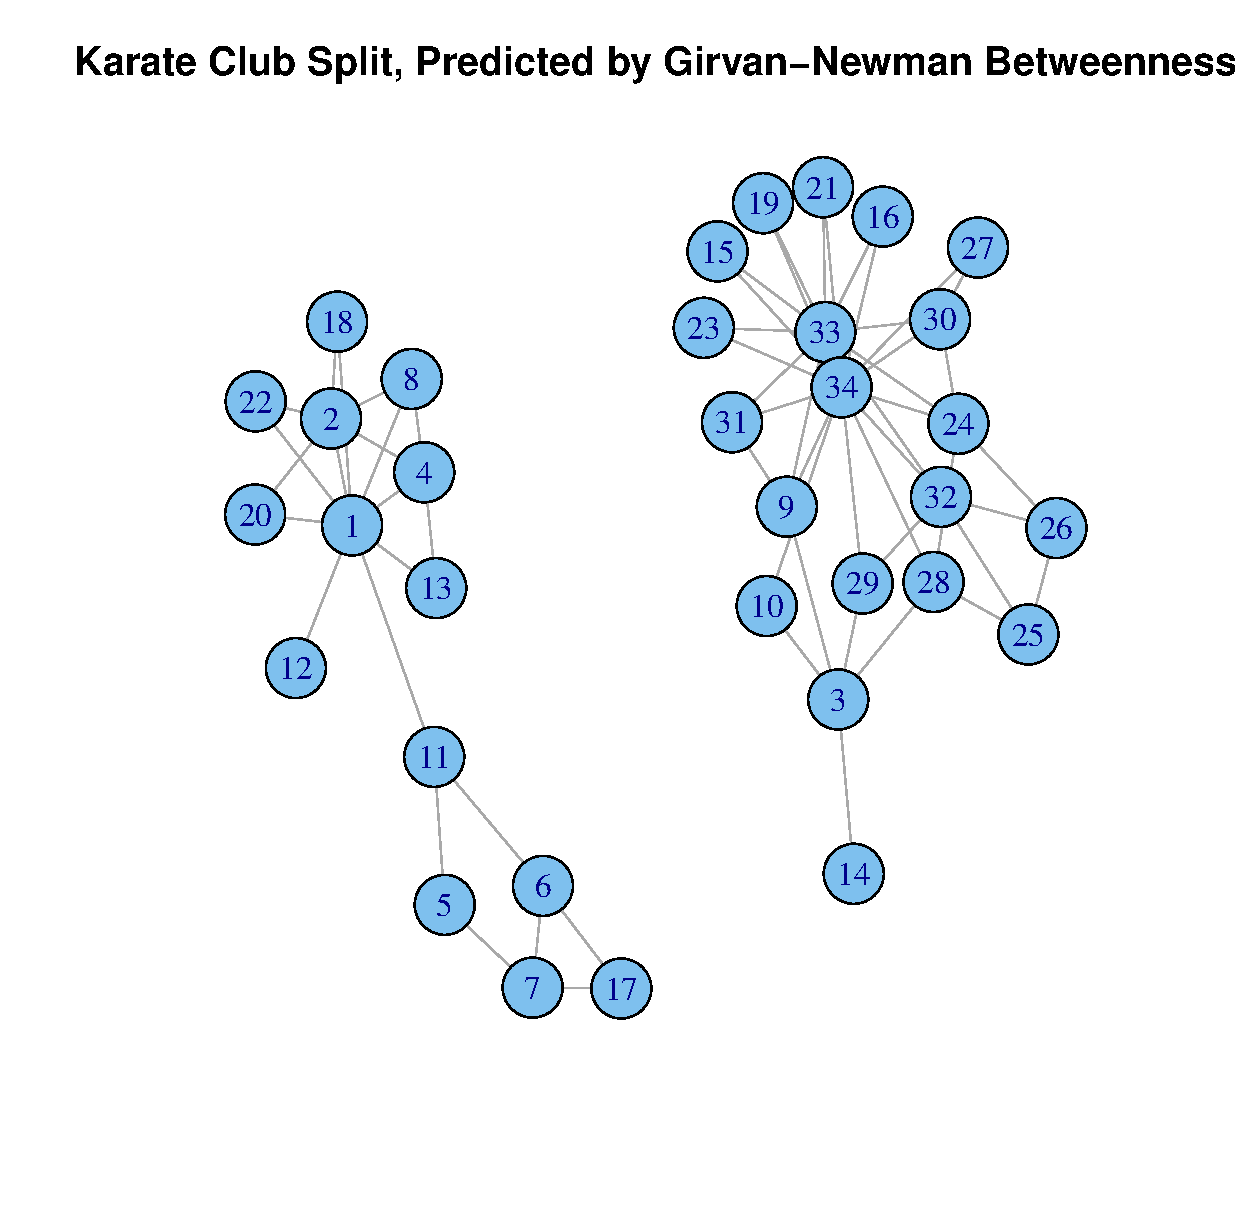
\includegraphics[scale=0.6]{R/kclub-gml-afterSplit.pdf}
\caption{Karate Club Graph Split Into 2 Groups Predicted by Girvan \& Newman Betweenness Clustering for ``karate.gml''}
\label{fig:after-split}
\end{figure}

\begin{figure}[h]
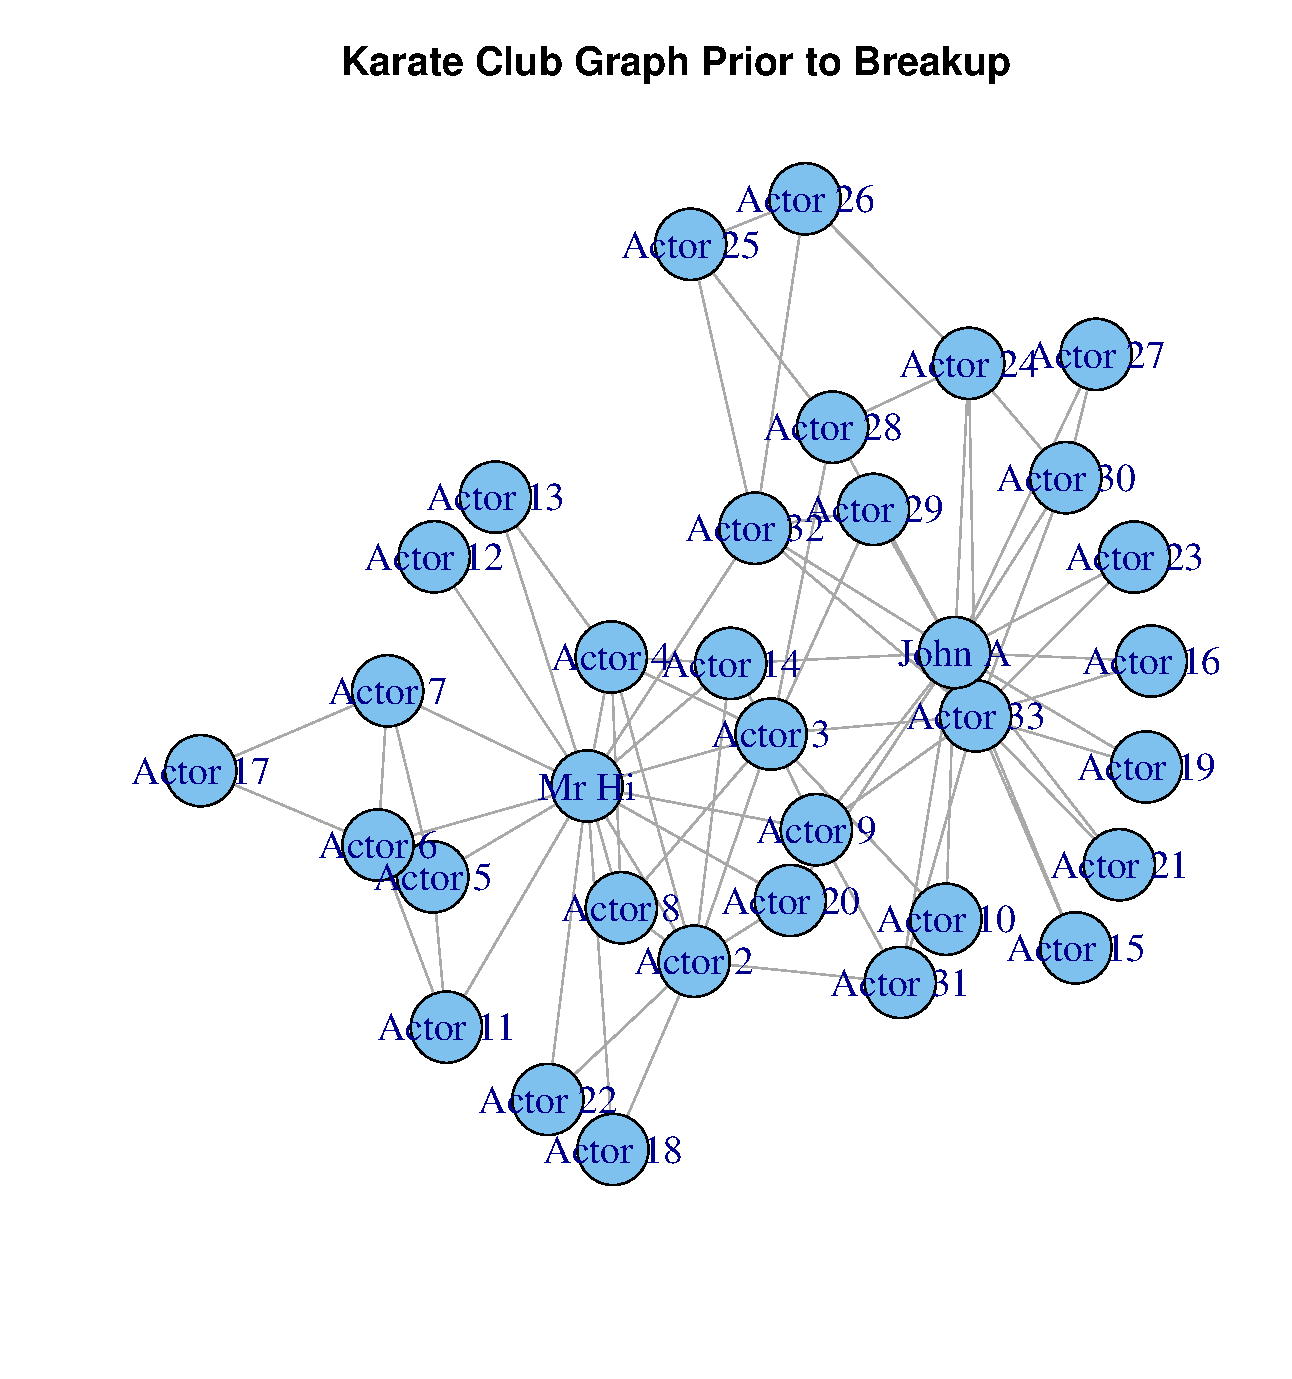
\includegraphics[scale=0.6]{R/kclub.pdf}
\caption{Karate Club Graph prior to split}
\label{fig:karate-before-split}
\end{figure}

\begin{figure}[h]
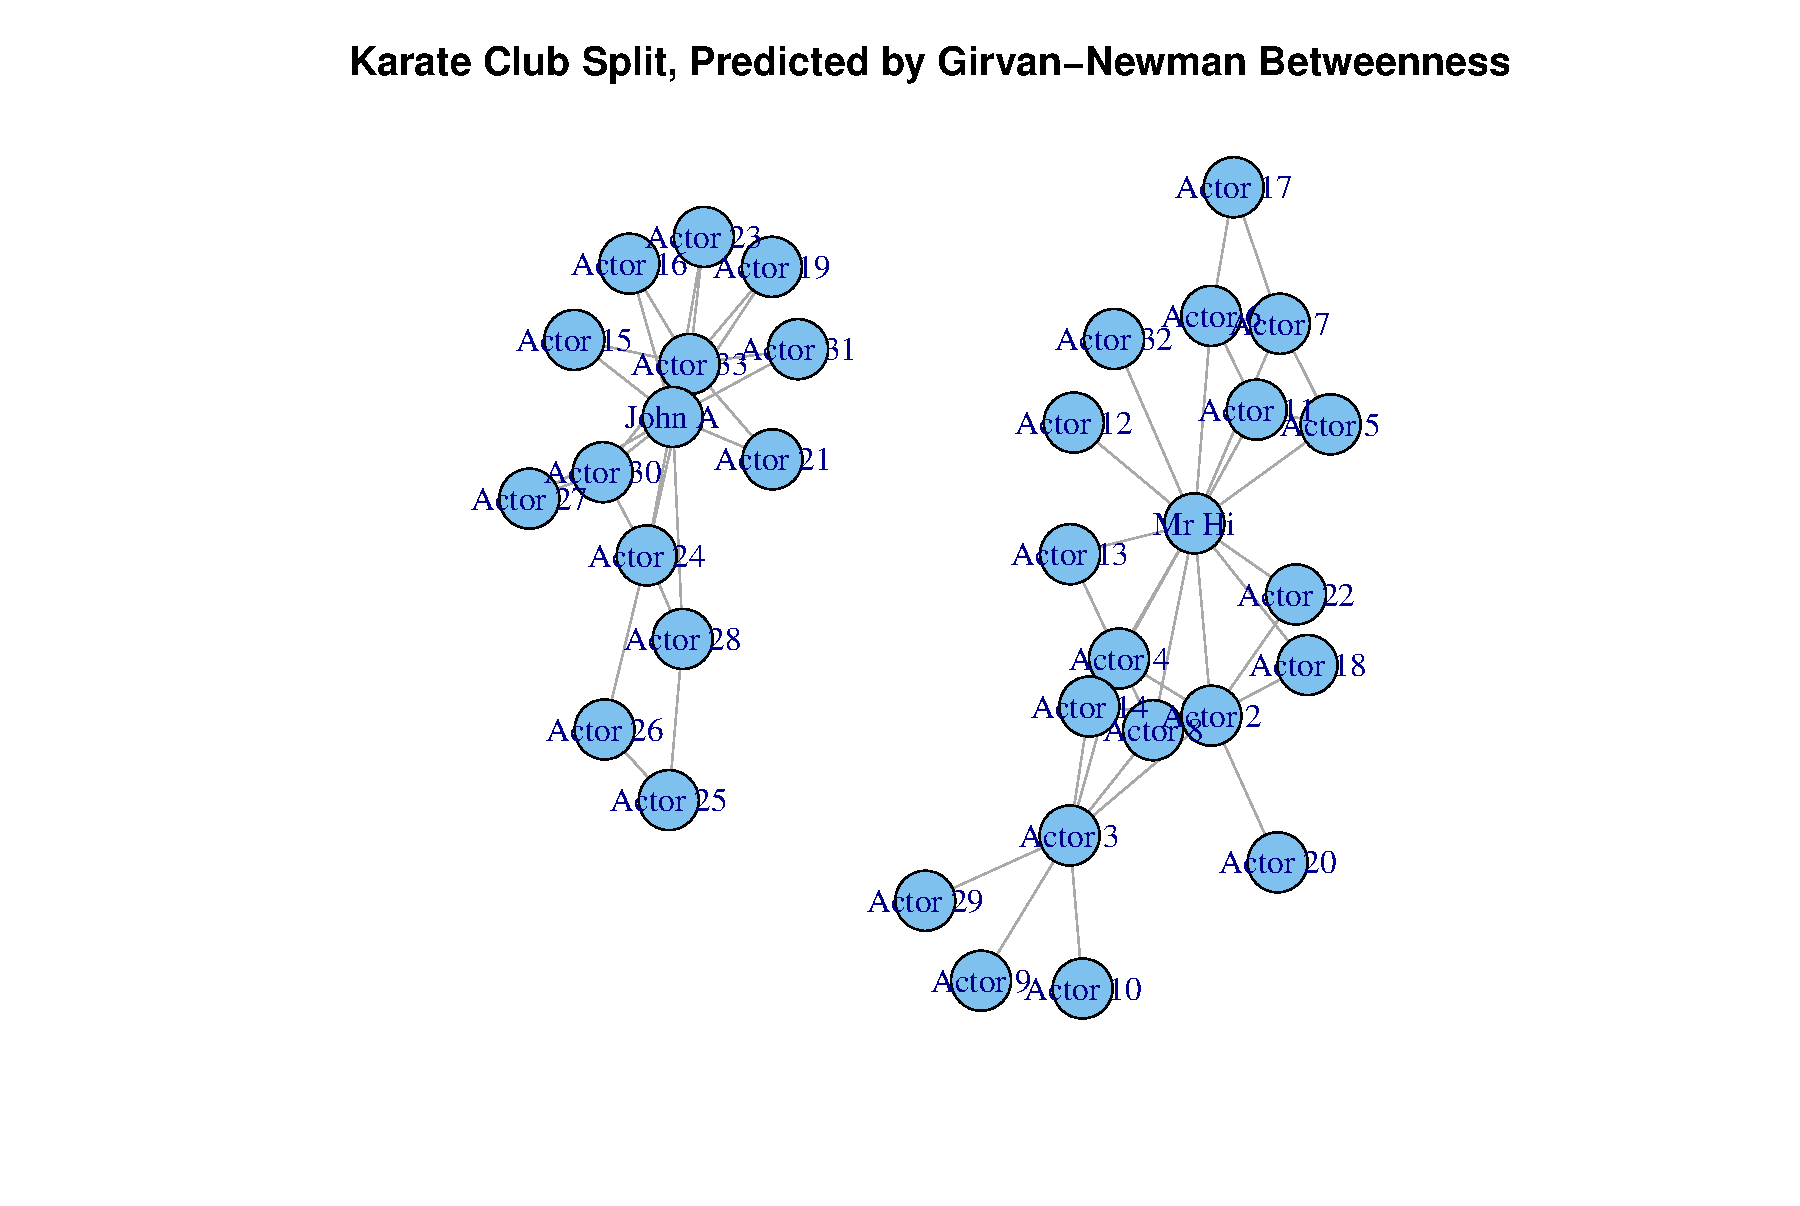
\includegraphics[scale=0.6]{R/kclub-into2.pdf}
\caption{Karate Club Graph Split Into 2 Groups Predicted by Girvan \& Newman Betweenness Clustering}
\label{fig:karate-after-split}
\end{figure}







